\documentclass[a4paper,times,12pt]{article}
\usepackage{amsthm}
\usepackage[figuresright]{rotating}
\usepackage{graphics}

\usepackage[utf8]{inputenc}
\usepackage[english]{babel}
\usepackage{graphicx}
\graphicspath{ {./images/} }
\title{trabalho-2-calculo-2}
\author{Public Domain}
\date{\today}

\usepackage{amssymb}
\usepackage{graphicx}
\usepackage{fancybox}
\usepackage{amsmath}
\usepackage{colortbl}
\usepackage{wasysym}
\usepackage{txfonts}
\usepackage{tikz}

\begin{document}

\hspace*{+15pt} 50. Calcular a área limitada pela curva \( r^{2} = 16 \cos{2 \theta} \).
\\
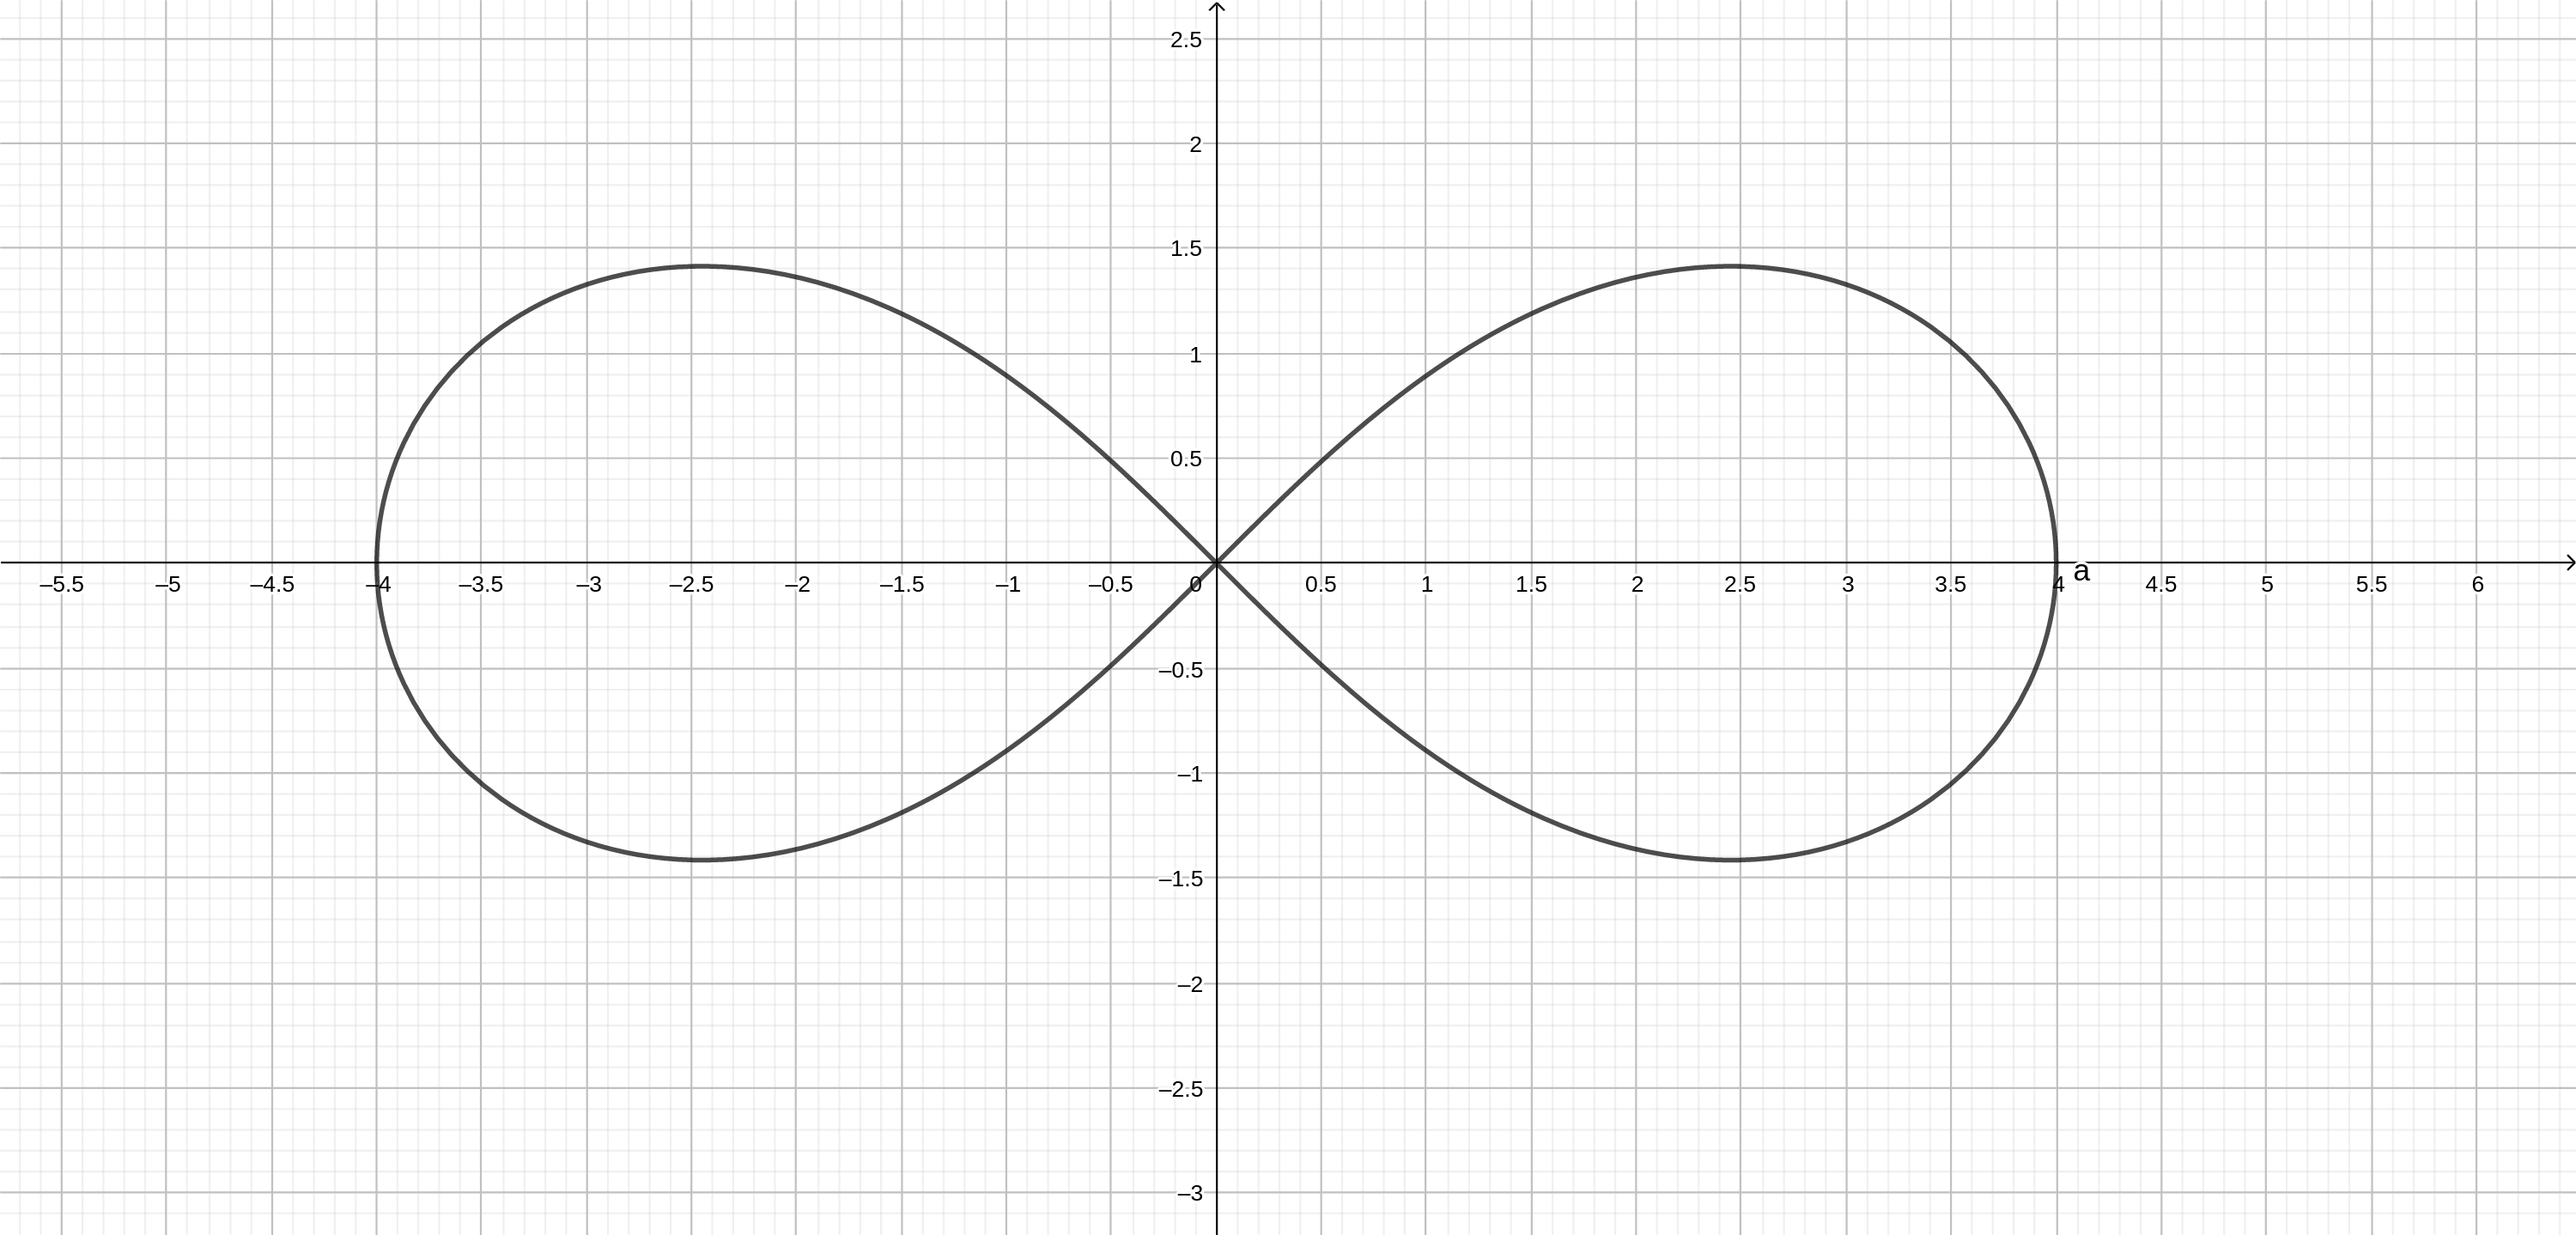
\includegraphics[width=\textwidth]{geogebra-export}
\\
\par Observando o gráfico dessa função, podemos observar simetria na origem. Portanto, para calcular a área, basta calcular a área de \( \alpha = 0 \) até \( \beta = \frac{\pi}{4} \) e multiplicar por 4.
\\
\par Aplicando a fórmula de área temos:
\[
	\frac{1}{2}4\int _0^{\frac{\pi }{4}}\left[\sqrt{16\cos 2\theta }\right]^2\:d\theta
\]
\par Simplificando temos:
\[
	\frac{1}{2}\cdot \:4\cdot \int _0^{\frac{\pi }{4}}16\cos \left(2\theta\right)d\theta
\]
\par Removemos a constante da integral:
\[
	\frac{1}{2}\cdot \:4\cdot 16\cdot \int _0^{\frac{\pi }{4}}\cos \left(2\theta\right)d\theta
\]
\par Resolvemos a integração:
\[
	\frac{1}{2}\cdot \:4\cdot 16\cdot\left[\sin \left(2\theta\right)\right]^{\frac{\pi }{4}_{0}}
\]
\[
	\frac{1}{2}\cdot \:4\cdot 16\cdot\left[\sin \left(2\left(\frac{\pi}{4}\right)\right)-\sin \left(2\left(0\right)\right)\right]
\]
\par Por fim, temos que:
\[
	\frac{1}{2}\cdot \:4\cdot 16\cdot1 = 16\ u.a.
\]

\end{document}